% !TEX TS-program = pdflatex
% !TEX encoding = UTF-8 Unicode

%%% DOCUMENT DEFINITIONS
\documentclass[11pt, french]{article} % use larger type; default would be 10pt
\usepackage[utf8]{inputenc} % set input encoding (not needed with XeLaTeX)

%%% PAGE DIMENSIONS
\usepackage{geometry} % to change the page dimensions
\geometry{a4paper} % or letterpaper (US) or a5paper or....
\geometry{margin=2cm} % for example, change the margins to 2 inches all round

%%% PACKAGES
\usepackage{graphicx} % support the \includegraphics command and options
\usepackage{booktabs} % for much better looking tables
\usepackage{array} % for better arrays (eg matrices) in maths
\usepackage{paralist} % very flexible & customisable lists (eg. enumerate/itemize, etc.)
\usepackage{verbatim} % adds environment for commenting out blocks of text & for better verbatim
\usepackage{subfig} % make it possible to include more than one captioned figure/table in a single float
\usepackage{amsmath}
\usepackage[frenchb]{babel}
\usepackage{eurosym} %pour le symbole euro
\usepackage[cdot]{SIunits}   % pour les unités (ohm,...)


\usepackage{picins,caption}
\usepackage{wrapfig}
\usepackage{url}

%%% HEADERS & FOOTERS
%\usepackage{fancyhdr} % This should be set AFTER setting up the page geometry
%\pagestyle{fancy} % options: empty , plain , fancy
% Rapport projet pluridisciplinaire : etude thermique du pont en H
% : Xavier Galzin, Stanislas Bertrand, Romain Desille, Frédéric Meslin

\title{\textsc{Projet Pluridisciplinaire} \\ Solution Numérique \\
\begin{minipage}[c][20cm][c]{15cm}
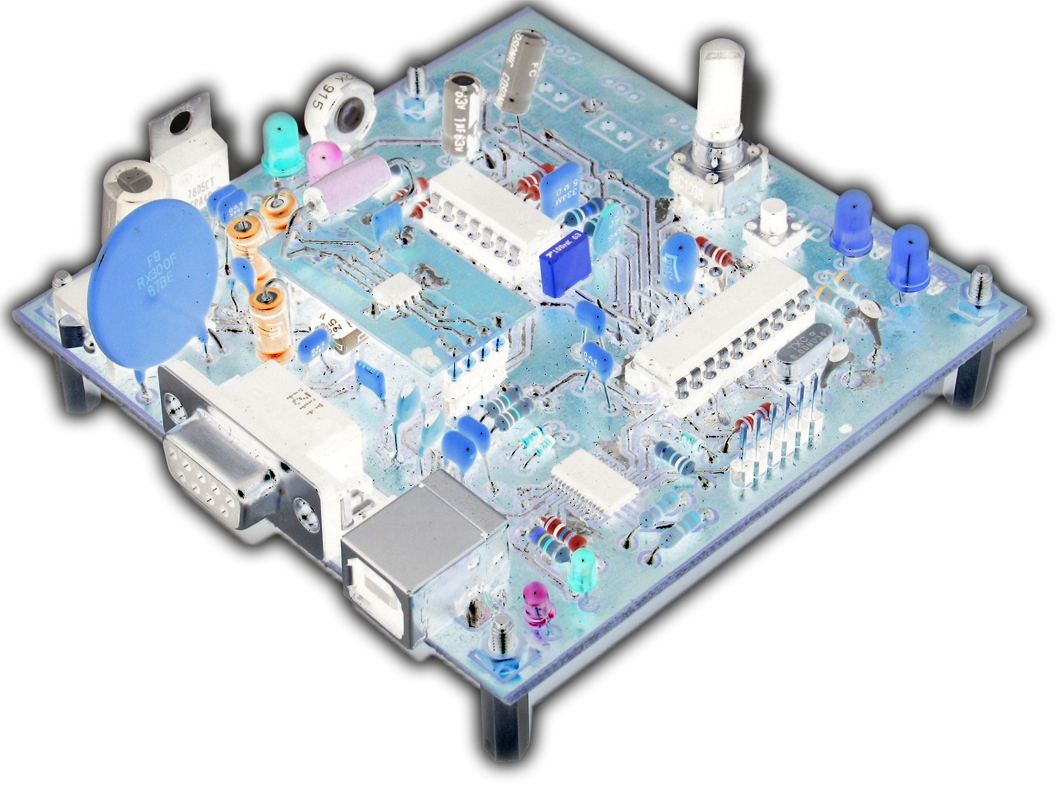
\includegraphics[width=15cm]{../Photos/CarteFrontInv.png}
\end{minipage}}
\author{Xavier GALZIN, Stanislas BERTRAND, Romain DESILLE, Frédéric MESLIN}
\date{\today}

\begin{document}
\maketitle

\pagebreak
\tableofcontents

\pagebreak
\section*{Introduction}
\addcontentsline{toc}{chapter}{Introduction}

Dans nos précédents rapports, nous avons détaillé le problème de l'asservissement en position du mobile et nous avons déterminé les paramètres d'un modèle analogique de correcteur. Par la suite, nous avons mis en place la théorie d'un protocole de communication série afin de faciliter les réglages et les mesures en temps réel. Dans le troisième rapport, nous avons décrit l'avancement de la partie analogique du projet, de la conception de la maquette jusqu'à sa réalisation et ses tests. 

\medskip

Dans ce dernier rapport, nous allons nous concentrer sur la correction numérique. Nous commencerons par définir les caractéristiques du protocole série que nous avons décidé d'utiliser en lieu et place de celui défini dans le rapport de MCSE, puis nous en expliciterons la programmation dans le microcontrôleur. Ensuite, nous aborderons brièvement la question de l'interface graphique mise en place et nous reviendrons également sur le changement intervenu dans la partie puissance avant de nous intéresser à la correction numérique à proprement parler. Enfin, nous clarifierons la question de la répartition des gains, en analogique comme en numérique, avant de conclure globalement sur le projet tout en proposant des possibilités d'améliorations que nous n'aurons malheureusement pas le temps de mettre en place. 


\section{Communication}
	La partie communication du projet peut paraître secondaire quand on considère l'application dans sa globalité. Pour quelles raisons un luminaire aurait-il besoin de communiquer avec un dispositif informatique ? L'intérêt semble limité ...

\medskip
Dans les faits, cette fonctionnalité a été implémentée dans une optique d'assistance au développement. Elle s'est avérée utile pour mettre au point l'asservissement numérique et faciliter le réglage des coefficients de la fonction de transfert du correcteur. Elle permet aussi désormais de collecter diverses informations liées à l'automatique pour analyser la qualité (stabilité) de l'asservissement. On imagine que cette liaison série ne sera pas intégrée dans le produit final, sauf si les spécifications devaient évoluer vers un appareil nécessitant de la connectivité. On peut penser à l'intégration dans un réseau domotique via des technologies Zigbee ou même au travers le Wifi.

La communication a aussi un intérêt pédagogique : nous avons fait le choix d'établir un protocole dédié sur une liaison de type série prise en charge par une connexion USB. Nous avons préféré cette solution à celle présentée dans la partie MCSE du projet pour plusieurs raisons qui vont être détaillées.

\subsection{Choix de la liaison USB}
	
Dans l'univers de la communication péri-informatique, la liaison USB est figure souveraine. La première version de cette spécification a vu le jour en 1996 dans l'objectif de remplacer progressivement les anciennes connectiques lentes et incompatibles entre elles.

\begin{wrapfigure}{r}{5cm}
	
\includegraphics[width = 4cm]{SolutionNumerique/usb-logo.jpg}
	\caption{Logo USB 2.0}
\end{wrapfigure}

\medskip
Ce document normalise à la fois : 
\medskip
\begin{itemize}
	\item un protocole complet de communication série maitre vers esclaves
	\item le matériel nécessaire pour faire transiter l'information (câble, prises ...)
	\item toutes les caractéristiques électriques et mécaniques associées
	\item des classes de pilotes standards couvrant un nombre important d'applications génériques.
\end{itemize}

\medskip
Notre application étant destinée à communiquer avec un ordinateur et l'USB fournissant une classe générique de communication série équivalente à un port COM virtuel, nous avons choisi d'opter pour cette solution.

\subsection{Utilisation d'un contrôleur USB - Série}

	Afin de bénéficier de la connectique USB sans entrer dans les détails de la sous-couche de communication, nécessitant des cycles de développement lourds, deux solutions s'offraient à nous :

\medskip
\begin{enumerate}
	\item Choisir un microcontrôleur disposant de fonctionnalités USB
	\item Utiliser un contrôleur USB externe
\end{enumerate}

\medskip
La première solution est la plus polyvalente car elle permet d'implanter n'importe quelle classe de périphérique dans le programme du microcontrôleur en se basant sur une bibliothèque USB fournie par le constructeur. Ceci nécessite une étude approfondie de la documentation associée et la rédaction de descripteurs USBs. Etant donné l'aspect auxiliaire de la communication, ce surcroit de développement a été écarté.

La seconde solution impliquant l'ajout d'un composant externe, au détriment du coût, a été retenue pour l'aisance de développement qu'elle apporte. Cette solution clef en main convertit une liaison série TTL en provenance du microcontrôleur en liaison USB de manière presque transparente.

\begin{figure}[h!]
	\centering
	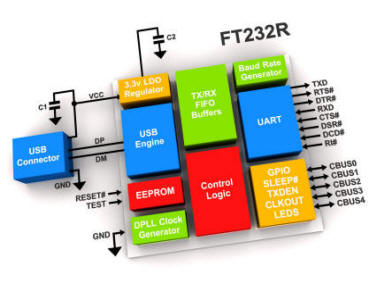
\includegraphics[width = 12cm]{SolutionNumerique/diagrammeFT232.jpg} 
	\caption{Diagramme interne du FT232}
\end{figure}

Le circuit contrôleur qui a été sélectionné est le FT232R de FTDI. Ce composant a été très simple à intégrer sur la carte du projet car il ne nécessite qu'une alimentation 5V et la liaison série pour fonctionner. De plus, il configure ses paramètres de transmission automatiquement en fonction de ceux communiqués par l'ordinateur à l'ouverture du port. Pour résumer ce composant est facile d'utilisation à défaut d'être peu couteux.

\subsection{Élaboration d'un protocole}
Dans le rapport de MCSE, nous avions présenté un protocole basique, exploitant un format de trames fixes de 3 octets consécutifs. Le premier contenant l'index de la commande et les deux suivants le corps de la donnée envoyée. Nous nous sommes rendus compte que ce protocole ne couvrait pas tous nos besoins et en particulier la possibilité de transmettre des messages d'erreurs ou de log.

\medskip
Nous avons donc programmé un autre protocole, plus évolué et plus évolutif. Celui ci est capable de transmettre plusieurs types de trames à longueur variable et d'inclure des codes de gestion d'erreur de transmission (au besoin).

\subsubsection{Configuration générale}
\noindent
Les paramètres généraux utilisés dans la transmission série sont les suivants :
\begin{description}
	\item[Taille donnée] 8 bits
	\item[Parité] Aucune parité
	\item[Bits de stops] 1 seul
	\item[Baudrate] variable de 9600 à 115200
\end{description}

\medskip
Le Baudrate est variable car le microcontrôleur dispose d'un module capable de déterminer automatiquement la vitesse de transmission de la liaison. La seule condition à respecter est l'émission du caractère ASCII "U" avant toute communication. Ce caractère correspond à un motif de niveaux logiques hauts et bas alternés qui permettent au périphérique série du microcontrôleur de calibrer son registre prescaler pour générer le bon Baudrate.

\subsubsection{Différentes trames}
\noindent
Nomenclature des symboles utilisés dans le protocole :

\medskip
\begin{description}
	\item[0] niveau bas logique
	\item[1] niveau haut logique
	\item[U] niveau indéfini (non interprété par le logiciel)
	\item[X] niveau à préciser selon l'utilisation
\end{description}

\medskip
\noindent
Les différentes trames disponibles sont les suivantes :
\medskip
\begin{itemize}
	\item\textbf{ Trame de contrôle :} \\

		\begin{tabular} {|c|c|c|c|c|c|c|c|}
			\hline
			\textbf{typ} & \textbf{r/w} & \textbf{chr} & \textbf{ad4} & \textbf{ad3} & \textbf{ad2} & \textbf{ad1} & \textbf{ad0}\\
			\hline
			1 & X &  X &  ad4 &  ad3 &  ad2 &  ad1 &  ad0 \\ \hline
		\end{tabular}

		\begin{description}
			\item[typ :] type de trame (0 : données | 1 : contrôle)
			\item[r/w :] type de transfert (0 : lecture | 1 : écriture)
			\item[chr :] type de données envoyées (0 : entiers 16 bits | 1 : chaine de caractères)
			\item[ad4 ... ad0] adresse de l'emplacement mémoire de la donnée (entière) envoyée (0 - 32)
		\end{description}

		La trame de contrôle est envoyée en premier et annonce une donnée entière ou une chaine de caractère. Elle est de type 0 pour la différencier des trames de données. Ceci permet de re-synchroniser la transmission en cas de perte d'un paquet de données. L'adresse de l'emplacement mémoire ne concerne pas les envois et réceptions de chaines.

\medskip
		En mode lecture (r/w = 0), le destinataire répond une trame de donnée entière ou plusieurs trames de chaine directement après réception de la trame de contrôle. En mode écriture (r/w = 1), la trame de contrôle doit être immédiatement suivie d'une trame de donnée entière ou de plusieurs trames de chaine.


	\medskip
	\item\textbf{ Trame de donnée entière :} \\

		\begin{tabular} {|c|c|c|c|c|c|c|c|c|}
			\hline
			\textbf{MSB :} & \textbf{typ} & \textbf{b06} & \textbf{b05} & \textbf{b04} & \textbf{b03} & \textbf{b02} & \textbf{b01} & \textbf{b00}\\
			\hline
			 & 0 & u &  u &  u &  d15 &  d14 &  d13 &  d12 \\ \hline
		\end{tabular}

		\begin{tabular} {|c|c|c|c|c|c|c|c|c|}
			\hline
			\textbf{MSB :} & \textbf{typ} & \textbf{b06} & \textbf{b05} & \textbf{b04} & \textbf{b03} & \textbf{b02} & \textbf{b01} & \textbf{b00}\\
			\hline
			 & 0 & u &  u &  u &  d11 &  d10 &  d09 &  d08 \\ \hline
		\end{tabular}

		\begin{tabular} {|c|c|c|c|c|c|c|c|c|}
			\hline
			\textbf{LSB : } & \textbf{typ} & \textbf{b06} & \textbf{b05} & \textbf{b04} & \textbf{b03} & \textbf{b02} & \textbf{b01} & \textbf{b00}\\
			\hline
			 & 0 & u &  u &  u &  d07 &  d06 &  d05&  d04 \\ \hline
		\end{tabular}

		\begin{tabular} {|c|c|c|c|c|c|c|c|c|}
			\hline
			\textbf{LSB : } & \textbf{typ} & \textbf{b06} & \textbf{b05} & \textbf{b04} & \textbf{b03} & \textbf{b02} & \textbf{b01} & \textbf{b00}\\
			\hline
			 & 0 & u &  u &  u &  d03 &  d02 &  d01 &  d00 \\ \hline
		\end{tabular}

		\begin{description}
			\item[typ :] type de trame (0 : données | 1 : contrôle)
			\item[d15 ... d00] valeur de la donnée 16 bits
		\end{description}

		Cette trame contient une donnée entière 16 bits à charger dans l'emplacement mémoire précisé dans la précédente trame de contrôle. On remarque que les bits b06, b05 et b04 ne sont pas utilisés. Ils peuvent être mis à profit pour intégrer un code détecteur d'erreur. Cette amélioration est envisageable dans une future version du projet.

	\medskip
	\item\textbf{ Trame de chaine de caractères :} \\

		\begin{tabular} {|c|c|c|c|c|c|c|c|}
			\hline
			\textbf{typ} & \textbf{r/w} & \textbf{log} & \textbf{ad4} & \textbf{ad3} & \textbf{ad2} & \textbf{ad1} & \textbf{ad0}\\
			\hline
			0 &  ch6 &  ch5 &  ch4 &  ch3 &  ch2 &  ch1 &  ch0 \\ \hline
		\end{tabular}

		\begin{description}
			\item[typ :] type de trame (0 : données | 1 : contrôle)
			\item[ch6 ... ch0] caractère table ASCII standard
		\end{description}

		Cette trame transmet une chaine de texte caractère par caractère. Pour distinguer les trames de données des trames de contrôle, on ne transmet que les 7 premiers bits de chaque caractère et on force le 8 ème à 0. Ce format autorise la représentation des caractères appartenant à la table ASCII standard mais pas à celle étendue. Pour terminer la transmission d'une chaine, il suffit d'envoyer une trame ne contenant que des zéros. Ceci équivaut à l'envoi du caractère de terminaison.

\end{itemize}

\subsection{Implantation du protocole}
Le présent protocole a été programmé dans la routine d'interruption de réception des données séries du microcontrôleur ainsi que dans l'application interface. Il rend possible des liaisons bidirectionnelles où le microcontrôleur comme l'application interface sont capables d'envoyer des trames de contrôle. En définitive, seul le sens application interface vers microcontrôleur a été implémenté, l'autre sens ne présentant que peu d'intérêt.

\section{Interface}
\subsection{Fonctionnement}
Afin de faciliter la phase de déboggage et pour régler pratiquement les paramètres du correcteur numérique, nous avons développé une petite application interface en C\char35. Le programme consiste en une simple fenêtre présentant une section de connexion, une section de configuration et un espace de texte pour afficher les messages de logs.

\begin{figure}[h!]
	\centering
	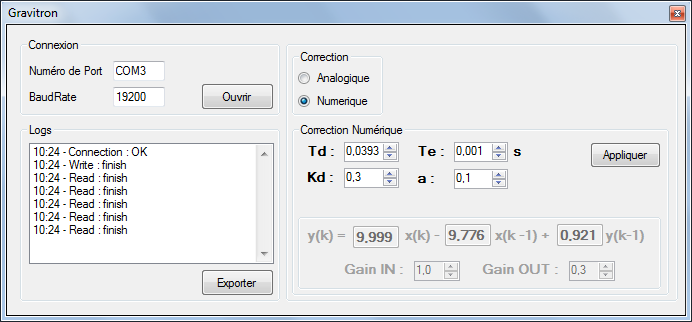
\includegraphics[width = 12cm]{SolutionNumerique/IHM.png} 
	\caption{Interface de l'application de contrôle}
\end{figure}

Le panneau de connexion requiert de l'utilisateur le choix du port série et la vitesse de transfert. Une fois la connexion établie, les autres sections grisées deviennent accessibles. 

La zone de messages logs liste chronologiquement les évènements de connexion et les messages textes envoyés par la maquette. Elle possède une fonctionnalité d'exportation permettant l'archivage des données dans un fichier texte.

Dès que la connexion entre le PC et la carte est établie, L'interface graphique demande le mode de correction en cours :  \textbf{analogique} ou \textbf{numérique}, on peut ensuite le modifier via les \textit{radiobuttons}. 
Par défaut, lorsque la carte démarre, c'est la correction analogique qui est mise en place. Pour passer en correction numérique, il faut donc se connecter avec un PC.

Lorsque la correction numérique est demandée, on lit dans un premier temps tous les paramètres de correction stockés dans le microcontrôleur puis on peut les modifier : \textit{$K_d$}, \textit{$T_d$}, \textit{$T_e$}, \textit{$\alpha$}. Il faut ensuite appliquer les changements avec un \textit{button}. A ce moment, les coefficients de l'équation de récurrence sont normalisés et envoyés au microcontrôleur. Une fois que ces différentes fonctionnalités ont été mises en place, nous nous sommes adonné à la réalisation de quelques "Gimmicks" décrits à la fin du rapport.

\subsection{Technologie utilisée}
Pour réaliser cette interface, nous avons utilisé Visual Studio 2010. C'est une application "Windows Forms" composée des différents objets du Framework Microsoft .NET 4. Visual Studio permet de réaliser des interfaces graphiques simples très rapidement, c'est pourquoi nous avons décidé d'utiliser ce dernier. 
Pour la communication série, nous utilisons l'objet "SerialPort" du Framework .NET, cet objet permet un accès rapide et sans trop de contraintes au port série.

Pour utiliser l'interface graphique, il faut donc installer le Framework .NET 4 qui est par défaut installé avec Windows 7.

\section{Changement de Puissance}

\subsection{Causes du changement}
Au cours de nos tests pour valider le fonctionnement de nos correcteurs analogiques et numériques, nous avons essayé de faire léviter le mobile à la distance de 1,5 cm. Nous avons eu du mal à y parvenir car notre pont en H chauffait de manière trop importante et la dissipation thermique était tout juste suffisante. La correction en résultant était donc assez instable bien que fonctionnelle. 

Nous avons donc voulu améliorer ce point en rajoutant un radiateur à notre pont en H. Cependant, ce dernier étant un composant CMS, il n'était pas possible d'ajouter facilement le radiateur. Nous avons alors tenté de coller le radiateur au plan de masse du dessous du circuit de puissance par le biais d'une grosse pastille d'étain. Malheureusement, notre pont en H CMS s'est dessoudé lors de l'opération.

Nous avons alors tenté de le ressouder en utilisant le four à refusion. Bien que cela ait fonctionné, il semble que la conduction thermique ait été très largement amoindrie. Il est également possible que le pont en H ait été endommagé lors de la seconde utilisation du four à refusion. Toujours est-il que le fonctionnement du pont est devenu encore moins satisfaisant qu'avant. C'est à ce moment que nous avons décidé de changer de pont en H, optant pour un composant Multiwatt afin de nous fournir une plus grande marge de manœuvre pour l'asservissement en augmentant le courant maximum utilisable. 

\subsection{Choix du nouveau pont en H}

Après consultation du catalogue Farnell, nous avons choisi un L6203 de ST Microelectronics. Bien qu'un peu plus cher (7.44 \euro{} en unitaire), ce composant fonctionne de manière similaire à l'A4950 : on peut choisir le sens de parcours du courant dans le pont par le biais des mêmes entrées qu'avec l'A4950. Cependant, ce composant nécessite des condensateurs de Bootstrap (1 par sortie) et supporte jusqu'à 5 A au lieu des 3,5 A du A4950. De plus, son boitier Multiwatt nous assure une dissipation thermique largement meilleure qu'avant en plus de nous permettre de rajouter facilement un radiateur. En outre, le $R_{DSON}$ de ce pont est de \unit{0,3}{\ohm} au lieu des 1,3 $\ohm$ de l'A4950 : on chauffera donc beaucoup moins tout en dissipant mieux, augmentant ainsi sensiblement notre marge de manœuvre pour l'asservissement. Enfin, le L6203 dispose également d'une protection thermique mais n'implémente plus de protection en courant. Il faudrait rajouter un comparateur sur la sortie $V_{Sense}$ du pont en H, ce que nous ne ferons pas pour des raisons de simplifications et à cause du fait que nous avons mis en place des protections empêchant un courant supérieur à 3 A de passer, ce qui est inférieur à ce que peut supporter notre pont. 


Ci dessous, le schéma bloc du L6203. 

\begin{figure}[h!]
	\centering
	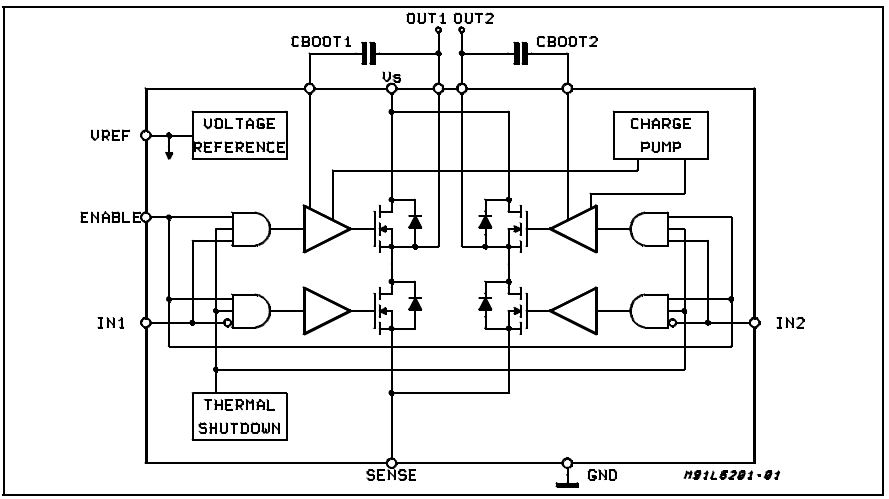
\includegraphics[width = 12cm]{SolutionNumerique/fonc_sch.png} 
	\caption{Schéma bloc interne du L6203}
\end{figure}

\subsection{Fonctionnement du L6203}

Après quelques mésaventures lors du routage (inversion de l'empreinte du pont en H), nous avons pu tester notre nouveau circuit de puissance. Celui-ci s'est avéré meilleur que le précédent, fournissant un asservissement plus stable en raison de sa plus grande tolérance aux plus grands courants. La consommation a également été diminuée (entre 0,4 et 0,5 A) grâce à la baisse significative du $R_{DSON}$. Il aurait été possible d'optimiser la consommation au détriment de la position en amenant le mobile de sorte que la répulsion du champ magnétique soit compensée par le poids du mobile. Ci-dessous le routage de la carte de puissance. 

\begin{figure}[h!]
	\centering
	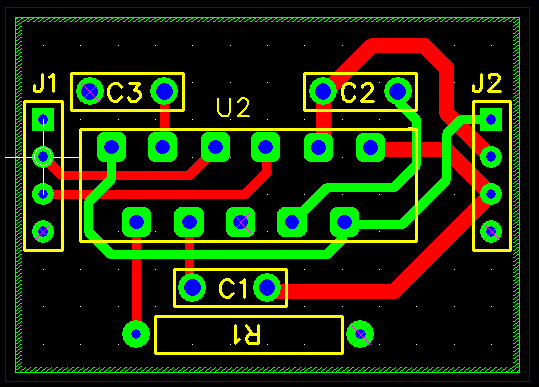
\includegraphics[width = 12cm]{SolutionNumerique/routage.png} 
	\caption{Routage de la carte de puissance}
\end{figure}

Sur ce routage, on voit bien les deux condensateurs de Bootstrap. La pin $V_{Sense}$ n'étant pas utilisée, on la relie à la masse (la résistance n'a pas été mise au final). La pin $V_{Ref}$ est une source de tension interne et nécessite d'être reliée à la masse par le biais d'un condensateur. 


\section{Correction Numérique}
\begin{wrapfigure}{r}{7cm}
		
	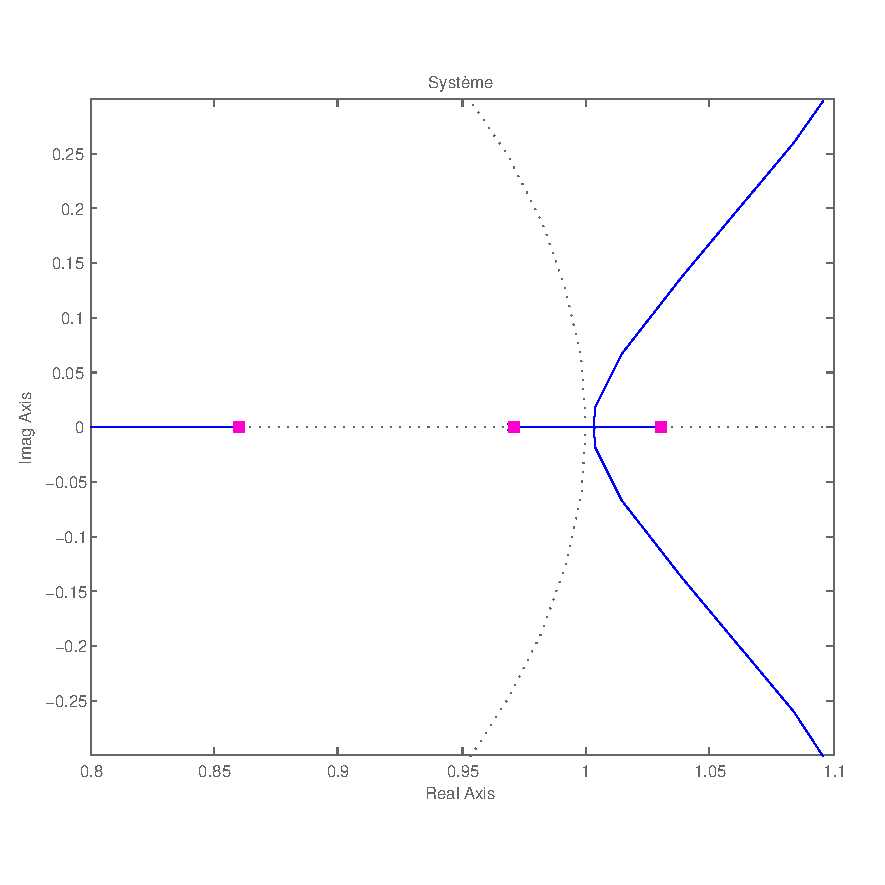
\includegraphics[width = 7cm,trim=0 1.4cm 0 1.2cm ,clip=true]
					{SolutionNumerique/Systeme.pdf}
	\caption{Système}
\end{wrapfigure}
La correction numérique découle du travail effectué pour la correction analogique. La sortie du montage différentiel est utilisée comme entrée du nouveau correcteur. La consigne analogique est la consigne utilisée dans cette correction.
Cette nouvelle solution est facile à implémenter et plus flexible. Les calculs réalisés pendant l'étude d'automatique du système donnent la forme du correcteur.

\[Co_{AvPh}(s)=\dfrac{1+ \tau_d \cdot s}{1 + a_d \cdot \tau_d \cdot s} \]

\[Co_{AvPh}(z)=\dfrac{a \cdot z + b}{z + c}=\dfrac{\dfrac{z}{a_d}+\dfrac{T_e-\tau_d}{a_d \cdot \tau_d} }{z+\dfrac{T_e-a_d \cdot \tau_d}{a_d \cdot \tau_d}}\] 

L'équation en $Z$ est obtenue avec une approximation des rectangles arrière, soit $s=\frac{z-1}{T_e}$. L'équation de récurrence en découlant implantée dans le microcontrôleur est $out_0=a \cdot in_0 + b \cdot in_1 + c \cdot out_1$. 
$in_1$ et $out_1$ sont le vieillissement des valeurs $in_0$ et $out_0$.

\begin{wrapfigure}{r}{7cm}

	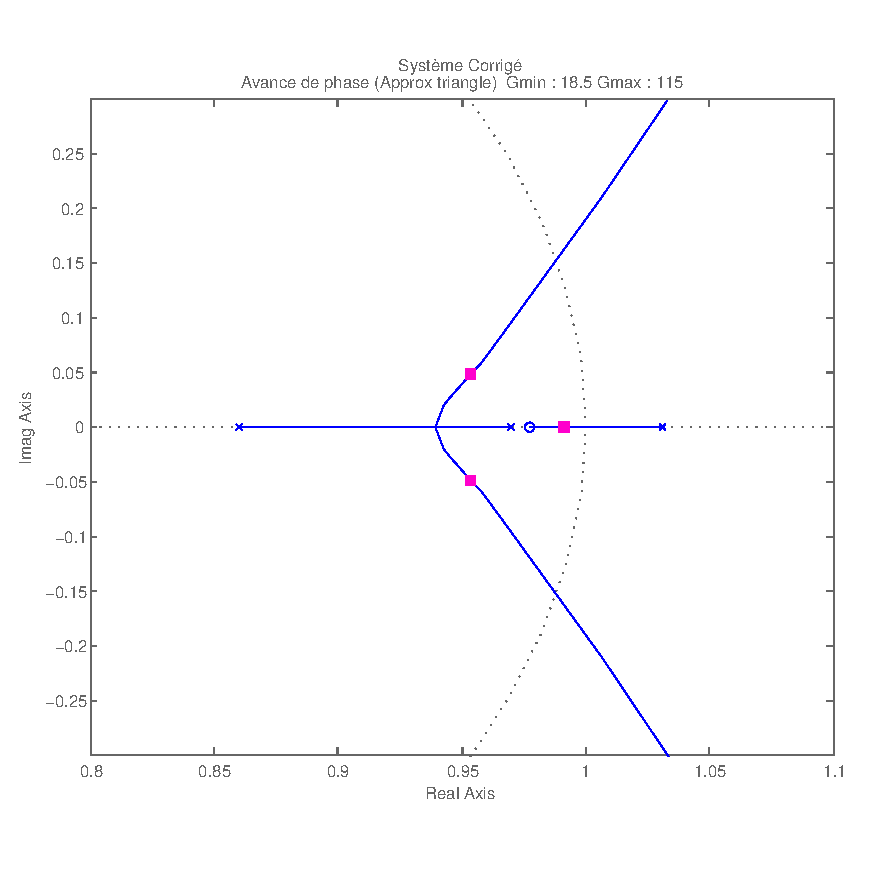
\includegraphics[width = 7cm,trim=0 1.4cm 0 0.7cm ,clip=true]
					{SolutionNumerique/SystemeCorrigeThorique.pdf}
	\caption{Système Corrigé Théorique}
	\vspace{1cm}
\end{wrapfigure}
Les valeurs des paramètres sont :

\[\tau_d=0.03934 \; T_e=0.001 \; a_d=0.1\]

La fréquence d'échantillonnage $T_e$ a été choisie par rapport à celle utilisée en analogique. La fonction de transfert correspondante est la suivante et donne le lieu d'Evans ci-contre.
\[Co_{AvPh}(z)=\dfrac{10 z - 9.776}{z -0.7756}\]

Lors des tests, les coefficients présentés ne permettent pas l'asservissement du mobile en position. Plusieurs causes sont possibles : la précision des calculs (virgule fixe, virgule flottante), le gain inadéquat ou encore des saturations en sortie.

L'asservissement en position a été obtenu en utilisant et adaptant les valeurs présentées dans le rapport d'automatique. Cependant ces valeurs correspondent à une fréquence d'échantillonnage de 1.7ms avec une approximation différente, le lieu d'Evans obtenu n'est pas celui recherché.
\[  Co_{AvPh_{Rapport Auto Modifie}}(z) = \dfrac {8.272z - 7.915} {z - 0.9} \]

La valeur $c=0.9$ a été modifiée par rapport au correcteur présenté dans le rapport d'automatique. Ce changement a pour effet de déplacer le pôle de l'avance de phase. On remarque alors que le gain théorique nécessaire pour la stabilité est de 5 contre 18.5 pour le correcteur précédent. Cependant la zone de stabilité théorique est très faible. Les oscillations observées lors des simulations confirment le résultat.

\begin{figure}[h!]
	\centering
	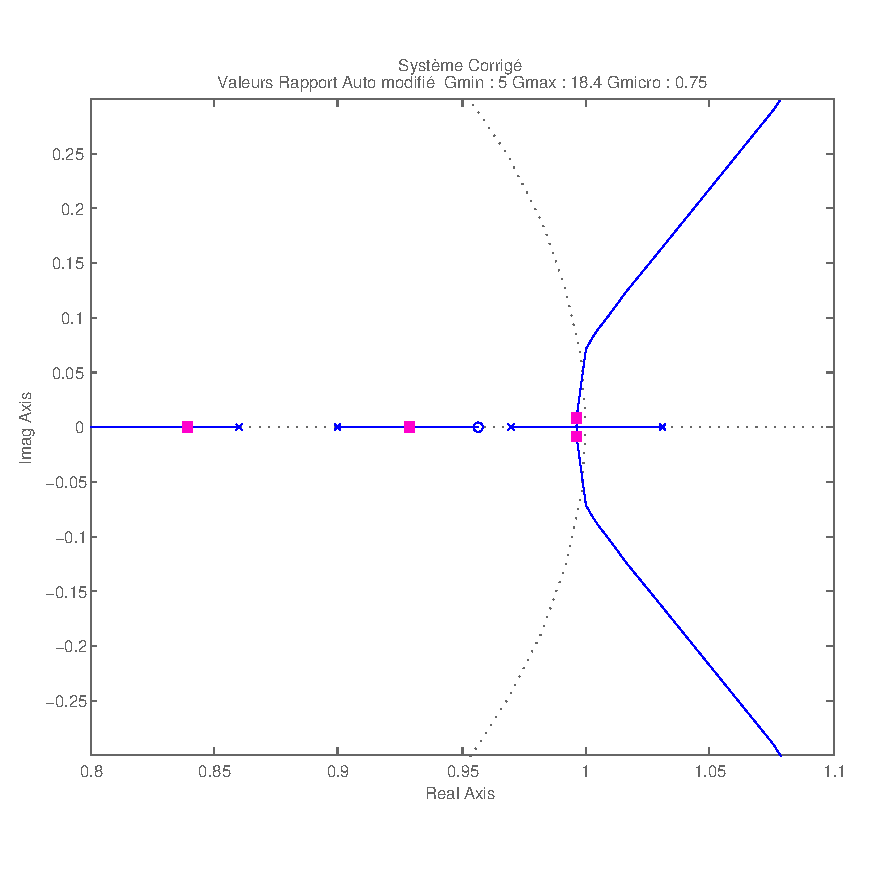
\includegraphics[width = 13cm,trim=0 1.4cm 0 0.7cm ,clip=true]
					{SolutionNumerique/SystemeCorrigeSolex.pdf}
	\label{CorrExpe}	
	\caption{Correction Expérimentale}
\end{figure}

Ce résultat apporte des réponses par rapport aux causes évoquées précédemment. Dans un premier temps, il est préférable d'effectuer les calculs en virgule flottante pour simplifier la mise en œuvre et observer le fonctionnement. Un surplus de gain occasionne des oscillations rapides mais le mobile lévite toujours, une saturation est peut-être présente quelque part et empêche un gain élevé.

\begin{wrapfigure}{r}{7cm}
	\vspace{-0.5cm}
	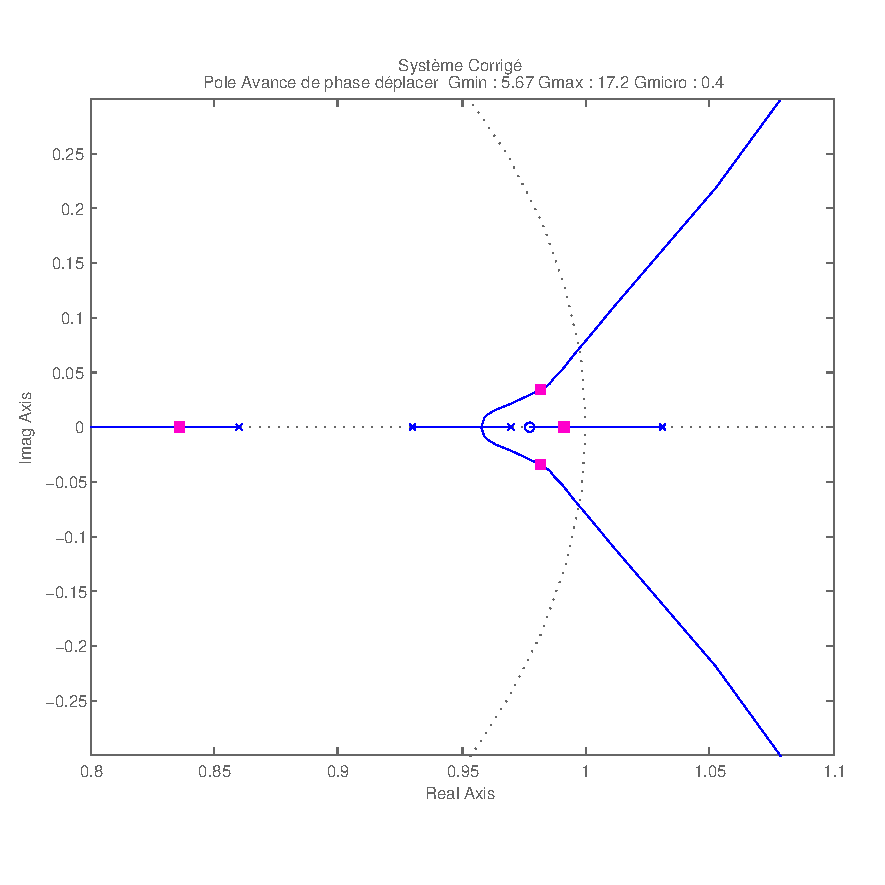
\includegraphics[width = 7cm,trim=0 1.4cm 0 0.7cm ,clip=true]
					{SolutionNumerique/SystemeCorrigeThoriqueAdapte.pdf}
	\caption{Correction Théorique Ajustée}
\end{wrapfigure}
Il est possible d'ajuster la correction théorique pour obtenir un gain équivalant à l'asservissement précédent et un meilleur comportement vis à vis des oscillations. La position du pôle du correcteur théorique est déplacée pour obtenir un gain théorique équivalant. 
\[  Co_{AvPh_{Theorique \; Modifie}}(z) = \dfrac {10z - 9.776} {z - 0.93} \]

L'amortissement du correcteur est plus important que précédemment. Les oscillations en lévitation sont moins importantes.

Le modèle utilisé pour l'élaboration des calculs théoriques est à relativiser, il est possible que la modélisation soit décalée par rapport notre système à cause d'imperfections de la bobine ou des capteurs.

%\vspace{+5cm}
%
%Difference avec le rapport d'auto
%-> Foh vers Zoh
%-> Fréquence de travail
%
%
%
%Questions / causes probables :
%-> est-ce que le gain de l'avance de phase compte ( analogique ) ?
%-> mauvais correcteur
%-> mauvais modèle
%-> mauvais calcul -> saturation, écretage, arondis
%
%Utilisation d'un outils :
%-> suivit des calculs via la série ( diff, avance de phase, sortie )
%
%dernière seance
%-> 1 gain du montage différentiel (3.5) (1+(2*R1)/R2) ==> /2 à cause des capteurs ==> 1,75
%	7k + 1k = 8k ==== 3.5 ---- 1.75 de gain
%-> 2 validation avec matlab de la répartition du gain ( av ph, num)
%	1.75*3*5 = 26.25 ok pour du analogique
%-> 3 validation avec l'asservissement numerique du mercredi du solex
%	1.75*4.5 = 7.875 numerique solex, oups manque le gain 5
%	1.75*5
%-> 4 essaye d'amélioration de l'asservissement numérique
%	pour un asservissement avec un zero correctement 


\section{Répartition des gains}

La répartition des gains le long de la chaîne d'asservissement est la suivante :
\begin{figure}[h!]
	\centering
	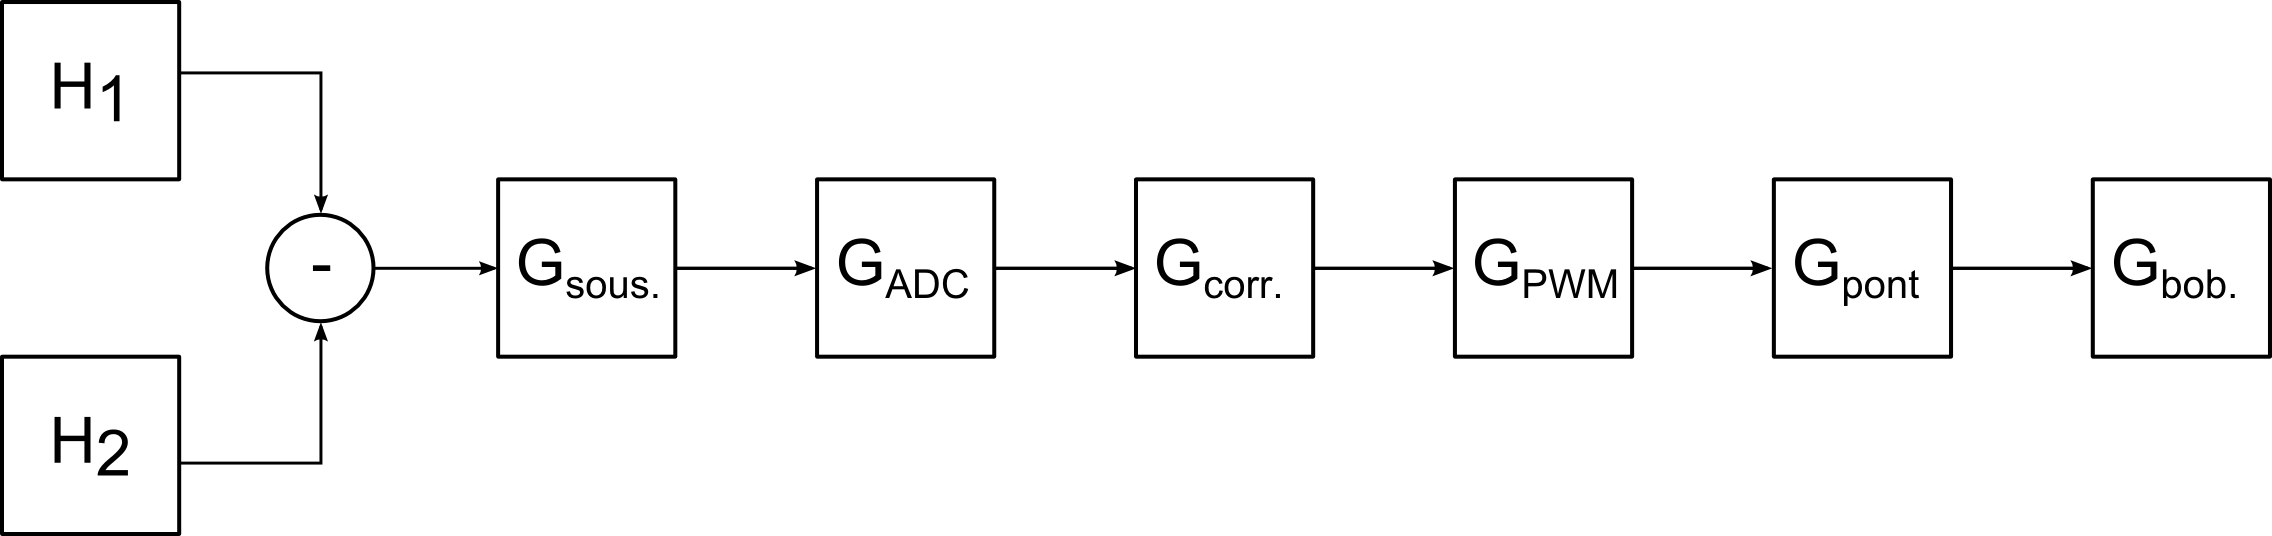
\includegraphics[width = 16cm]{SolutionNumerique/Gain.png} 
	\caption{Chaine automatique des gains}
\end{figure}

\pagebreak

\noindent 
\begin{enumerate}
\item[$G_{sous}$ : ]
Le gain du montage différentiel est donné par : \\ $G_{sous}=\frac{1}{2}\left( 1+2 \frac{R}{R0_{pot}+R0_{fix}}\right)$ avec $R=10k\ohm$, $R0_{pot}=7k\ohm$, $R0_{fix}=1k\ohm$ \\ ce qui donne $G_{sous}=1,75$.
\item[$G_{ADC}$ : ]
Le gain d'acquisition est : \\ $G_{ADC}= \frac{Plage \; de \; sortie}{Plage \; d'entr \acute{e} e}=\frac{4096}{5V}$, 5V en entrée représentée sur 12 bits. 
\item[$G_{Corr.}$ : ]
Le gain de correcteur est en fonction de l'asservissement utilisé.
\item[$G_{PWM}$ : ]
La PWM a deux modes, 9 bits et la plage représentée est 10V. \\ $G_{PWM}= \frac{Plage \; de \; sortie}{Plage \; d'entr \acute{e} e}=\frac{10V}{1024}$.
\item[$G_{Pont}$ : ]
Le pont transforme $\pm5V$ en $\pm12V$ ce qui donne $G_{pont}=2,4$.
\item[$G_{Bob}$ : ]
Le gain de la bobine est pris en compte dans le modèle du correcteur. 
\item[$G_{Total}$ : ]
Le gain total est alors de $33,6$.
\end{enumerate}

\subsection{Correcteur Analogique}
Pour la solution analogique, le gain du correcteur interne au microcontrôleur est de 1. Le système est stable pour le gain de boucle total bien que quelques oscillations puissent être perçues. Le gain du montage avance de phase n'est pas évoqué car il est pris en compte dans le modèle.
\subsection{Correcteur Numérique}
Les gains internes appliqués pendant les corrections numériques expérimentales et théorique ajustée sont de 0,75 et 0,4. Les gains de boucle ainsi obtenus sont respectivement 25,2 et 13,44. Le gain obtenu pour la première correction ne correspond pas au modèle qui possède un gain maximal de 18.4, cependant le mobile lévite. D'autre part, pour la correction théorique ajustée, le gain interne de 0.4 est une valeur limite basse ce qui ne concorde pas avec le gain élevé de 13,44 proche de la limite théorique du modèle de 17,2.

Il existe des correspondances floues entre les gains expérimentaux et ceux théoriques. Une analyse approfondie sur les calculs réalisés dans le microcontrôleur et des plages d'entrée des valeurs serait nécessaire et possible grâce à la liaison série.

\section{Gimmicks}
 
 En plus des asservissements numériques et analogique, nous avons mis en place trois fonctionnalités additionnelles :
 
 \medskip
 
 - La première est d'ordre pratique. En temps normal, dès que l'on cesse d'asservir, le mobile chute. Cela provoque un bruit plutôt désagréable (et  accessoirement on casserait l'ampoule dans le cas d'une lampe). Nous avons donc implémenté une fonctionnalité qui amène le mobile à se coller à la bobine lorsque l'on quitte l'application graphique. 
 
 - Seconde fonctionnalité : tant que l'on est en analogique, on acquiert les mesures via la liaison série. Il est possible d'exporter ces mesures au format CSV afin de générer des courbes pour y suivre l'évolution de la position du mobile.
 
  - La dernière est d'ordre artistique : lorsque le mobile vient se coller sur la bobine, on joue un air de musique connu \footnote{http://www.youtube.com/watch?v=Kh2AWswAMvw} est faisant varier la fréquence de la PWM dans la bobine avec un rapport cyclique de 50\%. 
  
\begin{figure}[h!]
	\centering
	
\includegraphics[width = 4 cm]{SolutionNumerique/mario.png} 
	\caption{Un air connu ?}
\end{figure}
 
\section*{Conclusion - Évolution}
\addcontentsline{toc}{chapter}{Conclusion - Évolution} 

Au cours de ce projet, nous aurons eu l'occasion de mettre en œuvre les connaissances que nous avons acquises pendant les semestres précédents. Nous sommes ainsi parvenus à concevoir une correction adaptée à notre système grâce à une étude d'automatique. Ensuite, en utilisant nos connaissances en électronique, nous avons réalisé ce correcteur ainsi que la boucle d'asservissement du système en choisissant nous-mêmes les composants nécessaires. Enfin, grâce à nos cours de microcontrôleur et de programmation, nous avons pu générer la PWM qui contrôle la bobine. Nous avons également mis en place une communication série asynchrone par USB avec un protocole de log pour envoyer et recevoir des données du microcontrôleur en plus de pouvoir gérer la correction numérique par le biais d'une interface graphique développée en C\#. 

\medskip

En termes de résultats, nous sommes parvenu à faire léviter le mobile aussi bien par un asservissement analogique qu'avec un asservissement numérique pour une consommation de l'ordre du demi Ampère. La communication série et l'interface sont fonctionnels et il est possible de passer sans difficultés de la correction analogique à la correction numérique en cours de fonctionnement. 

\medskip

Plusieurs améliorations peuvent encore être envisagées pour perfectionner notre solution :

- Le contrôle de la consigne par le biais de l'interface graphique : nous avons envisagé d'implémenter cette fonctionnalité peu avant la dernière séance. Cependant, à cause de la manière dont la consigne analogique est généré, il est nécessaire d'effectuer des modifications hardware pour parvenir à gérer la consigne numériquement. Nous n'avons pas voulu risquer de compromettre le fonctionnement de notre solution en effectuant de telles modifications.

- L'affichage de courbes : avec davantage de temps, nous aurions pu afficher des courbes de position du mobile ou de valeur de PWM (reflétant la consommation) sur l'interface graphique

\pagebreak
\section*{Annexes}
\addcontentsline{toc}{chapter}{Annexes}

Les codes microcontrôleur et les codes de l'IHM seront fournis dans une archive séparée. 

\begin{figure}[h!]
	\centering
	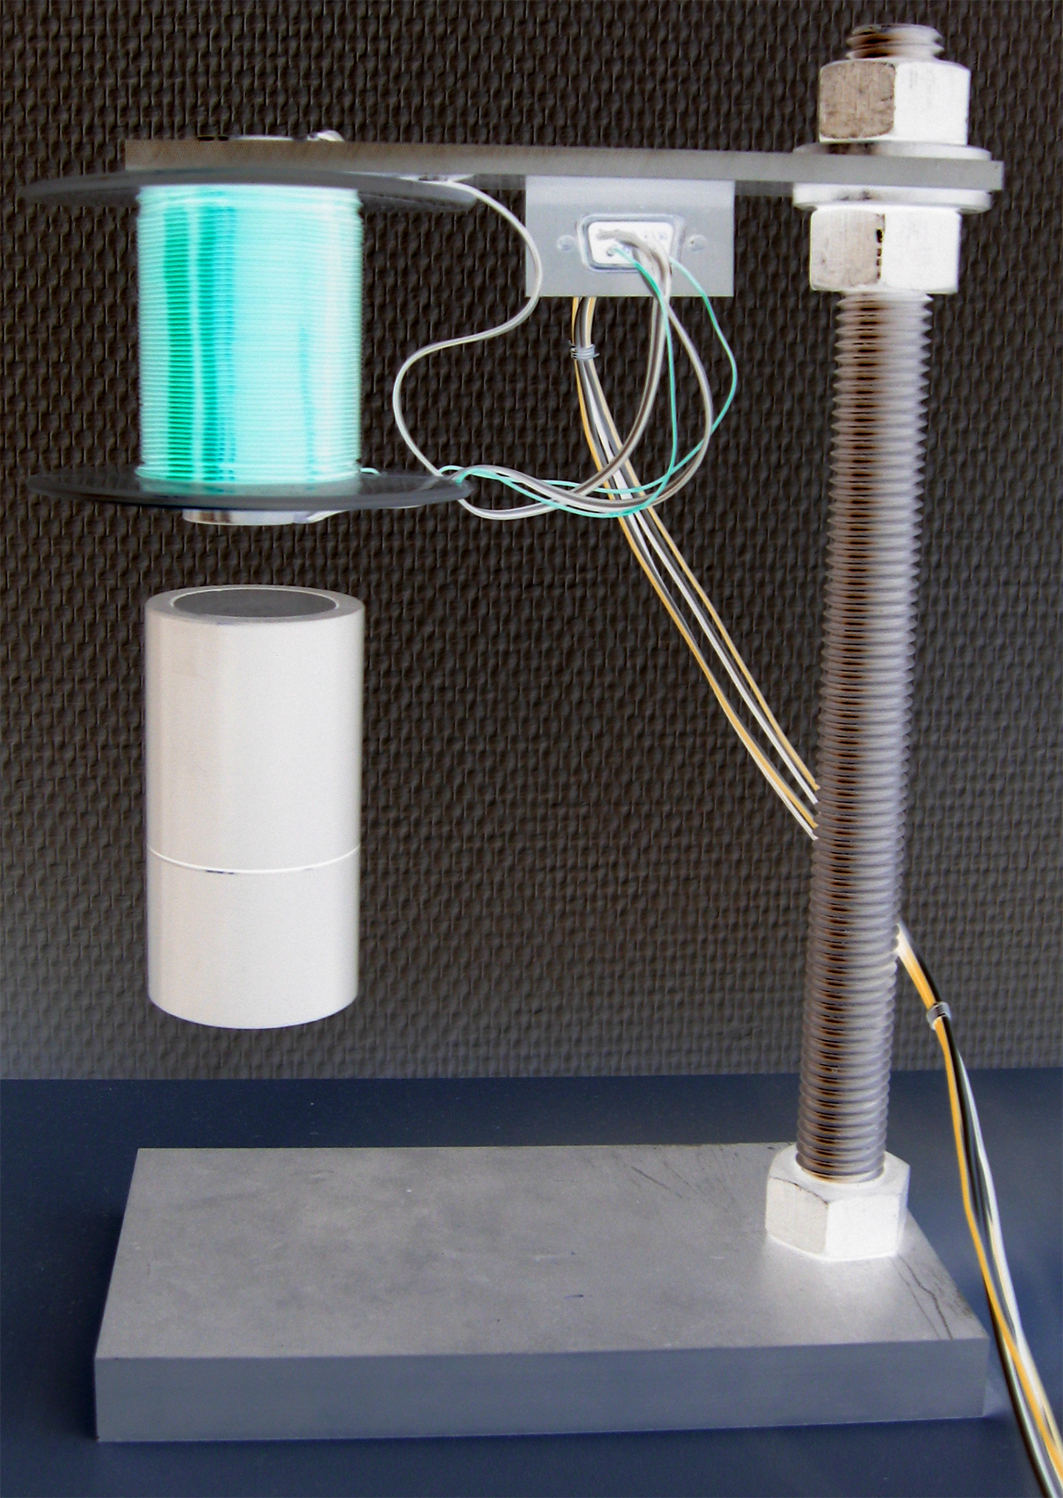
\includegraphics[width = 12 cm]{SolutionNumerique/levitation.png} 
	\caption{Tadaaa !}
\end{figure}
 

\end{document}

